\subsection*{\hypertarget{adv}{Adventuring}}
\addcontentsline{toc}{subsection}{Adventuring}
"Why not? Nothing to lose but my life... and I got that for free!"
\indent -- Setzer

\begin{center}
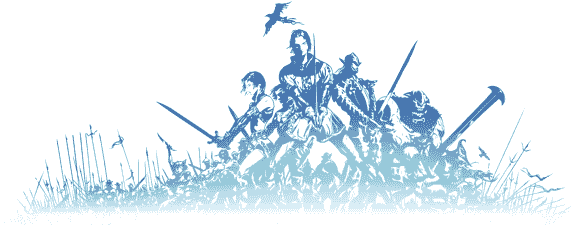
\includegraphics[width=\columnwidth]{./art/images/ff11.png} 
\end{center}

\vspace{0.1cm}

\subsubsection*{\hypertarget{check}{Checks}}
Checks are the main tool to help the GM to decide and narrate the outcome of actions.
He can either ask players for checks or perform them himself in secret.
Checks are usually \textbf{2d} rolls and higher numbers mean a better outcome for the roller. 
The minimum result required to succeed is called Difficulty~(shortened \textbf{DC}) and often has to be decided by the GM.
He should base this DC on the difficulty of the action and the proficiency of the actor in it.
Since checks are 2d rolls, the lowest and highest possible results are 2 and 12 respectively, which can be treated as unexpectedly good or bad, but plausible outcomes.
A check can also have \textbf{Advantage} or \textbf{Disadvantage} when the environment substantially affects the attempted action. 
In both cases the check is made with 3d and with Advantage only the two highest and with Disadvantage only the two lowest dice are counted. 
The table below shows rough categories for DCs.

\vfill

\begin{tcolorbox}[colback=white, tabularx={@{\hspace{1cm}} p{0.5\columnwidth} p{0.3\columnwidth}},sharp corners=south,colframe=accent, 
	title=\begin{center}\textbf{Difficulty Categories}\end{center}]	
	\textbf{Action} 	& \textbf{DC} \\
	\hline 	Very Hard 	& 11 - 12 \\
	\hline	Hard 		& 8 - 10 \\
	\hline  Medium 		& 5 - 7 \\
	\hline  Easy 		& 1 - 4 \\
\end{tcolorbox}

\vfill

\example{Checks}
{
Cloud meets Don Corneo in his mansion wearing a dress and make-up to convince him that he is a woman.
The GM decides that this is a very difficult task (DC 11), because Cloud did not put much effort into his disguise. 
But as the room is not well lit and the Don had a bit too much to drink, he also decides that the check has Advantage. 
Cloud rolls 3d with the result [6,2,6] and since only the two highest dice count, he rolled the best possible outcome! 
The GM decides that Don Corneo is not only convinced that Cloud is a woman, but he finds him so irresistible that he drags Cloud into his room for some time alone.
}

\pagebreak

\subsubsection*{Exploration}
The party can explore the environment described by the GM at will.
They can look for specific objects or wander around, but an appropriate amount of time passes while doing so.
The GM may draw a map of the party's current location as a visual aid. 
He is also free to impose checks on all exploration related actions, such as picking locks or detecting traps.
The party may go to sleep once per day to fully recover their HP and MP, even if unconscious.
To gain this benefit, they have to sleep in a comfortable place like an Inn or a \hyperlink{item}{Tent} for multiple hours.

\vfill

\subsubsection*{Social Interaction}
Throughout the adventure, the party will interact with other characters.
These non-player characters are voiced by the GM and accordingly the players talk from the perspective of their own characters.
To avoid confusion, it is important to clarify whether something you say is from the perspective of your character or from yours as player or GM.
During conversations, the GM may ask for checks, for example to decide whether attempt to convince a character is successful.

\vfill

\subsubsection*{Experience}
Characters become stronger by gaining experience and we express the amount of experience a character has with \textbf{Levels}.
Inexperienced adventurers start at Level 1 and can progress up to a maximum of Level 10 where they become renowned heroes. 
The GM decides when characters Level up, which we recommend for reaching adventure \mbox{\textbf{\hypertarget{ms}{Milestones}}}.
Such Milestones are for example important character development events, victories against powerful foes, or resolution of major conflicts. 

\vfill

\subsubsection*{Death}
When going on dangerous adventures, death is always a real possibility, especially as a consequence of unwise decisions by the party. 
The adventure is officially over if all party members fall \textbf{unconscious} in battle, as this is usually followed by certain death. 
Characters may also die or leave the party under special circumstances in which case that character becomes unplayable for their player. 

\vspace*{0.7cm}

\example{Experience \& Death}
{
	Kain betrays the party and joins their enemies. 
	He duels his friend Cecil and defeats him and the rest of the party in combat, but chooses to let them stay alive.
	The GM takes control of Kain from now on, who leaves the party and becomes an antagonist.
	The party resolves to stop Kain's plan and his former player decides to create a new character that joins the party. 
	The GM rewards the party with a Level up for reaching a turning point in the adventure.
}

\pagebreak
